\documentclass{report}
\usepackage[a4paper]{geometry}
\usepackage[myheadings]{fullpage}
\usepackage{fancyhdr}
\usepackage{lastpage}
\usepackage{graphicx, wrapfig, subcaption, setspace, booktabs}
\usepackage[T1]{fontenc}
\usepackage[font=small, labelfont=bf]{caption}
\usepackage{fourier}
\usepackage[protrusion=true, expansion=true]{microtype}
\usepackage[english]{babel}
\usepackage{sectsty}
\usepackage{url, lipsum}
\usepackage{float}
\usepackage{gensymb}
\usepackage{amsmath}
\graphicspath{ {./images/}}


\newcommand{\HRule}[1]{\rule{\linewidth}{#1}}
\onehalfspacing
\setcounter{tocdepth}{5}
\setcounter{secnumdepth}{5}
\setcounter{MaxMatrixCols}{20}
%-------------------------------------------------------------------------------
% HEADER & FOOTER
%-------------------------------------------------------------------------------
\pagestyle{fancy}
\fancyhf{}
\setlength\headheight{15pt}
\fancyhead[L]{Stephen Chen}
\fancyhead[R]{UBID: 50225769}
\fancyfoot[R]{Page \thepage\ of \pageref{LastPage}}
%-------------------------------------------------------------------------------
% TITLE PAGE
%-------------------------------------------------------------------------------

\begin{document}
\title{ \normalsize \textsc{ }
		\\ [2.0cm]
		\HRule{1pt} \\
		\LARGE \textbf{Rocket Design and Fly}
		\HRule{1pt} \\ [0.5cm]
		\normalsize  \vspace*{5\baselineskip}}



\author{Stephen Chen \\
	Student ID: 50225769 \\ 
	University at Buffalo \\
	MAE 423 Final Project \\
}
        
        
\date {May 11, 2021}


\maketitle
\tableofcontents
\newpage

%-------------------------------------------------------------------------------
% Section title formatting
\sectionfont{\scshape}
%-------------------------------------------------------------------------------

%-------------------------------------------------------------------------------
% Problem Statement
%-------------------------------------------------------------------------------

\section*{Problem Statement}
\addcontentsline{toc}{section}{Problem Statement}

The purpose of this final project is to explore the process of designing and testing sounding rockets given the desired design specifications using contraints based on trajectory theory, propulsion systems, structural strength of materials, and flight stability.
To build the rockets, a number of inputs will be required to define the rocket's physical shape and properties.
By comparing and analyzing the flight properties of the resultant rockets with their input parameters, we shoul de able to determine how input parameters affect the properties of the rocket.
To simplify and limit the infinite number of designs that are possible when designing a rocket, the following basic geometry is followed for all of the rockets built.

\begin{figure}[h!]
    \centering
    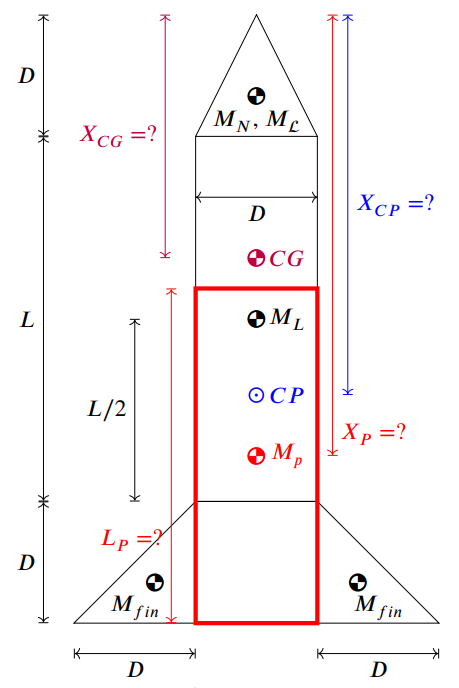
\includegraphics[height = .31\textheight]{./figures/rocketShape.png}
    \caption{Basic Rocket Geometry}
    \label{fig:rocketgeo}
\end{figure}

\noindent By following this basic geometry, a rocket's design can be defined by only two design parameters, length L, and diameter D.\\

\noindent Other design parameters that are necessary in defining the physical properties of the rocket are the following:\\

\begin{table}[h]
    \centering
    \caption{Rocket Design Specifications}
    \begin{tabular}{|c|c|c|}
        \hline
        \textbf{Design Specifications} & \textbf{Value} & \textbf{Description}\\
        \hline
        $M_L$  & 5 & Payload mass [kg] \\[5pt]
        $h_{max}$ & 10k, 20k, 30k & Maximum altitude [ft] \\[5pt]
        $a^*_{max}$ & 5, 10, 20 & Normalized max. acceleration \\[5pt]
        $SM$ & 1, 2, 3 & Static margin \\[5pt]
        $\rho_s$ & 1820 & Shell density [$\frac{kg}{m^3}$] \\[5pt]
        $\rho_p$ & 1772 & Propellant density [$\frac{kg}{m^3}$] \\[5pt]
        $\sigma_s$ & 80 & Shell working stress [MPa] \\[5pt]
        $N$ & 4 & Number of fins \\[5pt]
        \hline
    \end{tabular}
    \label{table:designspec}
\end{table}

\noindent From Table \ref{table:designspec}, we can see that some values remain constant while others include a selection.
The constant values include the payload mass located in the cone of the rocket, the shell density, propellant density, shell working stress, and number of fins.
The values that include a selection are the values that will be changed when designing the various rocket cases.\\

\noindent To configure the rocket for each case, we must decide on a diameter and length for the rocket.
Since the rockets can be built in any size with any precision, this could also result in an infinite number of rockets.
To limit and choose the best rocket configuration for each case, we will be iteratively testing each rocket sizing for flight stability and maximizing the payload coefficient. \\

\noindent A computer program was written in Python to automatically create and test rockets for each design case by creating millions of rockets with varying diameter and lengths. 
The diameter of the rockets ranged from 0.001m to 3m in 0.001m increments. 
The length of the rockets ranged from 0.001m to 5m in 0.001m increments.
With these sets of design parameters, the program could create 15 million different sizing configurations for each case. \\

\noindent With the specification options shown in Table \ref{table:designspec}, we can see that a total of 27 configurations can be created.
However, to make the data more simple and easier to analyze, a total of 9 cases will be generated instead. 
To accomplish this, when selecting the parameters from the selections, the other two parameters are set to the medium option.
For example, if we want to generate a design case of $h_{max} = 30k$, then $a^*_{max} = 10$ and $SM = 2$.
The cases conducted are shown in Table \ref{table:designcase}.\\

\begin{table}[h!]
    \centering
    \caption{Rocket Design Specifications}
    \begin{tabular}{|c|c|c|c|}
        \hline
        \textbf{Cases} & \textbf{$h_{max}$} & \textbf{$a^*_{max}$} & \textbf{SM}\\
        \hline
        1 & 10k & 10 & 2 \\[4pt]
        2 & 20k & 10 & 2 \\[4pt]
        3 & 30k & 10 & 2 \\[4pt]
        \hline
        4 & 20k & 5 & 2 \\[4pt]
        5 & 20k & 10 & 2 \\[4pt]
        6 & 20k & 20 & 2 \\[4pt]
        \hline
        7 & 20k & 10 & 1 \\[4pt]
        8 & 20k & 10 & 2 \\[4pt]
        9 & 20k & 10 & 3 \\[4pt]
        \hline
    \end{tabular}
    \label{table:designcase}
\end{table}

\newpage
\section*{Method of Solution}
\addcontentsline{toc}{section}{Method of Solution}

The program starts by calculating $R_{opt}$, $W_{eq}$, and $t_b$ with the design specification variables using the equations below.
These equations are viable because we are assuming a linear burn with the chemical propellant.

\begin{equation}
    R_{opt} = a^*_{max} + 1
\end{equation}

\begin{equation}
    W_{eq} = \sqrt{\frac{h_{max}g}{\frac{ln(R_{opt})}{2}[ln(R_{opt}-2)]+\frac{R_{opt}-1}{R_{opt}}}}
\end{equation}

\begin{equation}
    t_b = \frac{(R_{opt}-1)W_{eq}}{gR_{opt}}
\end{equation}

\noindent where $R_{opt}$ is the optimal mass ratio, representing the ratio of initial to burnout mass of the rocket, $W_{eq}$ is the equivalent velocity of the rocket, and $t_b$ is the burnout time.
These values can then be used to calculate the equivalent Mach number $M_{eq}$ and total pressure $P_0$ within the rocket's combustion chamber.
The speed of sound and atmospheric pressure was found assuming that the rocket is fired and travels near the surface of the Earth. 
With this assumption, the speed of sound and atmospheric pressure becomes: 

\begin{equation}
    a = 346 [\frac{m}{s}]
\end{equation}

\begin{equation}
    P_a = 101325 [Pa]
\end{equation}

\begin{equation}
    M_{eq} = \frac{W_{eq}}{a}
\end{equation}

\begin{equation}
    P_0 = \frac{P_a}{(1+\frac{\gamma-1}{2}M^2_{eq})^{\frac{-\gamma}{\gamma-1}}}
\end{equation}

\noindent where $\gamma = 1.4$ is the specific heat ratio of air.\\

\noindent Then, after guessing the diameter of the rocket, the thickness of the rocket shell can be calculated using the hoop stress equation shown below with $\sigma_s$ being the working stress of the rocket shell.

\begin{equation}
    \delta = \frac{DP_0}{2\sigma_s}
\end{equation}

\noindent After guessing the length of the diameter, we can calculate the mass of the rocket shell, mass of the rocket propellant, and length of the propellant tank.
The equations used to calculate them are shown below.
The mass of the rocket shell is calculated by simplifications including assuming the thickness of the shell is much less than the diameter ($\sigma_s << D$).
We also assume the fins are the same thickness as the shell.

\begin{equation}
    M_{s,cone} = \frac{\pi D}{2}\Biggl(\frac{D}{2}+\sqrt{D^2+(\frac{D}{2})^2}\Biggr)\delta\rho_s
\end{equation}

\begin{equation}
    M_{s,body} = \pi D(L+D)\delta\rho_s
\end{equation}

\begin{equation}
    M_{s,fin} = \frac{D^2}{2}\delta\rho_s
\end{equation}

\begin{equation}
    M_s = M_{s,cone} + M_{s,body} + NM_{s,fin}
\end{equation}

\begin{equation}
    M_p = (R_{opt}-1)(M_s+M_L)
\end{equation}

\begin{equation}
    L_p = \frac{4M_p}{\pi D^2 \rho_p}
\end{equation}

\noindent The location of the center of pressure $X_{cp}$ and center of gravity $X_{cg}$ are calculated with the following equations. 
See Appendix for derivation of $X_{cp}$ and $X_{cg}$.

\begin{equation}
    X_{cp} = \frac{\frac{4}{3}\Biggl[L+\biggl[\frac{16}{1+\sqrt{1+(2.5D)^2}}\biggr](L+\frac{3D}{2})\Biggr]}{2+\frac{4}{3}\biggl[\frac{16}{1+\sqrt{1+(2.5D)^2}}\biggr]}
\end{equation}

\begin{equation}
    X_{cg} = \frac{(M_{s,cone}+M_L)(\frac{2D}{3})+M_{s,body}(D+\frac{L+D}{2})+M_p((2D+L)-\frac{L_p}{2})+NM_{s,fin}(L+\frac{5D}{3})}{M_{s,cone}+M_{s,body}+M_p+NM_{s,fin}}
\end{equation}





\newpage
\section*{Discussion of Results}
\addcontentsline{toc}{section}{Discussion of Results}

After successfully configuring the 9 rocket cases, the results can be seen in Table \ref{table:caseresult1} and Table \ref{table:caseresult2} below.

\begin{table}[h!]
    \centering
    \caption{Rocket Case Configuration Results 1}
    \begin{tabular}{|c|c|c|c|c|c|c|c|}
        \hline
        \textbf{Cases} & $R_{opt}$ & $W_{eq}$ [m/s] & $t_b$ [s] & $P_o/P_a$ & $\delta/D$ & D [m] & L/D \\
        \hline
        1 & 11 & 146.871 & 13.611 & 1.132 & 7.168e-4 & 0.168 & 8.226 \\
        2 & 11 & 207.708 & 19.248 & 1.276 & 8.079e-4 & 0.165 & 10.073 \\
        3 & 11 & 254.389 & 23.574 & 1.432 & 9.071e-4 & 0.172 & 6.401 \\
        \hline
        4 & 6 & 304.075 & 25.830 & 1.653 & 1.047e-3 & 0.139 & 8.151 \\
        5 & 11 & 207.708 & 19.248 & 1.276 & 8.079e-4 & 0.165 & 10.073 \\
        6 & 21 & 153.368 & 14.889 & 1.144 & 7.247e-4 & 0.212 & 7.604 \\
        \hline
        7 & 11 & 207.708 & 19.248 & 1.276 & 8.079e-4 & 0.203 & 3.975 \\
        8 & 11 & 207.708 & 19.248 & 1.276 & 8.079e-4 & 0.165 & 10.73 \\
        9 & 11 & 207.708 & 19.248 & 1.276 & 8.079e-4 & 0.143 & 18.434 \\
        \hline
    \end{tabular}
    \label{table:caseresult1}
\end{table}

\begin{table}[h!]
    \centering
    \caption{Rocket Case Configuration Results 2}
    \begin{tabular}{|c|c|c|c|c|c|c|c|}
        \hline
        \textbf{Cases} & $X_{CG}$ & $X_{CP}$ & $M_p$ & \textbf{$M_s$} & \textbf{$M_o$} & \textbf{$\lambda$} & \textbf{$\epsilon$} \\
        \hline
        1 & 0.972 & 1.308 & 52.074 & 0.207 & 57.281 & 9.564e-2 & 3.967e-3 \\
        2 & 1.194 & 1.524 & 52.598 & 0.260 & 57.858 & 9.460e-2 & 4.915e-3 \\
        3 & 0.749 & 1.093 & 52.335 & 0.233 & 57.568 & 9.512e-2 & 4.441e-3 \\
        \hline
        4 & 0.794 & 1.072 & 25.852 & 0.170 & 26.022 & 1.921e-1 & 6.547e-3 \\
        5 & 1.194 & 1.524 & 52.598 & 0.260 & 57.858 & 9.460e-2 & 4.915e-3 \\
        6 & 1.127 & 1.551 & 107.936 & 0.397 & 113.333 & 4.615e-2 & 3.663e-3 \\
        \hline
        7 & 0.701 & 0.904 & 52.481 & 0.248 & 57.730 & 9.482e-2 & 4.706e-3 \\
        8 & 1.194 & 1.524 & 52.598 & 0.256 & 57.858 & 9.459e-2 & 4.915e-3 \\
        9 & 1.828 & 2.257 & 52.821 & 0.282 & 58.093 & 9.416e-2 & 5.311e-3 \\
        \hline
    \end{tabular}
    \label{table:caseresult2}
\end{table}

\noindent We can see from the tables above that changing the design specification parameters affected multiple properties of the resultant rocket.
Cases 1-3 show us that by increasing the $h_{max}$, the equivalent velocity $W_{eq}$, burnout time $t_b$, pressure ratio $P_o/P_a$, and thickness ratio $\delta/D$ also increases.
This trend makes sense because to reach higher velocities, the rocket must be propelled for longer.
This causes the equivalent velocity, burnout time and pressure ratio to increase.
Then, to contain the increased pressure of the combustion chamber, the thickness of the shell must also increase.\\

\noindent From analyzing cases 4-6, we can see that by increasing the normalized acceleration $a^*_{max}$, the mass ratio $R_{opt}$, diameter $D$, propellant mass $M_p$, and overall mass $M_o$ of the rocket also increased.
We can also see that $\delta/D$, $W_{eq}$, $t_b$, $P_o/P_a$, payload ratio $\lambda$, and structural ratio $\epsilon$ decreased with increased acceleration.
These results make sense because to get increased thrust and acceleration, the burnout time of the rocket must decrease along with the equivalent velocity.
$R_{opt}$ is directly calculated from the normalized acceleration so it increases.
The decreased equivalent velocity means lower pressure ratio which leads to thinner shell thickness. 
The mass of the propellant must increase drastically, to more than four times that of the lowest acceleration case compared to the highest, to propel enough mass for the increased acceleration.
Because of this, the rocket also requires more shell material (more than double) and increased the total mass of the rocket.
We can also see that due to the increased mass while payload mass remains constant, the payload ratio drastically decreased to about 25\%. \\

\noindent Analyzing cases 7-9, we can see that changing the static margin $SM$ does not affect the rocket's flight properties.
However, it does affect the size of the rocket greatly. 
By increasing the static margin of the rocket, the length, CG location, CP location, and structural ratio also increased.
The rocket's diameter and payload ratio decreased with increasing static margin. 
This result tells us that by increasing the static margin of the rocket, the resultant rocket will have to be skinnier, with larger L and smaller D. 
Because of this, the location of the center of gravity and center of pressure must move with the increased length.
The mass of the propellant also inreased slightly (\textasciitilde0.6\%), most likely due to the slightly increased shell mass and overall mass due to the longer rocket body.
The structural ratio increased by a larger percentage (\textasciitilde12.9\%) because the shell mass increased more than the propellant mass, \textasciitilde13.7\% compared to \textasciitilde0.6\%.\\

\begin{figure}[h!]
    \centering
    \fbox{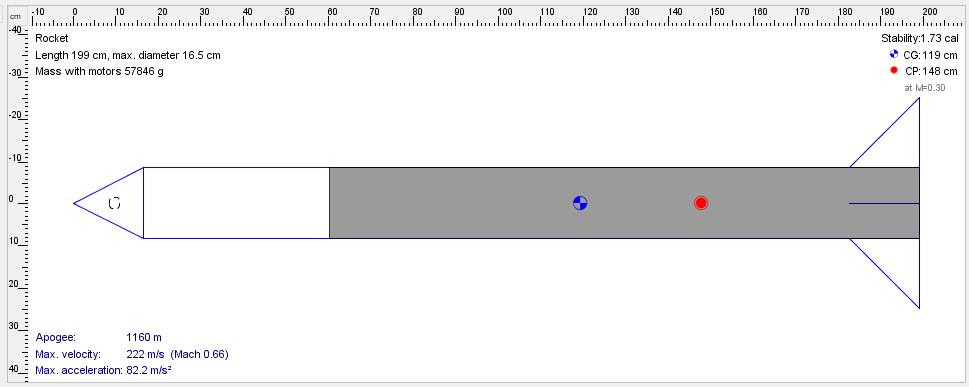
\includegraphics[width = 0.8\textwidth]{./figures/rocketDesign.png}}
    \caption{OpenRocket Design Based on Configuration Case 5}
    \label{fig:rocketDesign}
\end{figure}

\noindent Figure \ref{fig:rocketDesign} above shows the design of the rocket for case 5 created in the OpenRocket software.
By comparing the CG and CP location from the figure to that of Table \ref{table:caseresult2}, we can see that the center of gravity location is off by \textasciitilde0.3\% and center of pressure location is off by \textasciitilde2.97\%.
This tells us that our program calculates the CG and CP locations correctly and matches the OpenRocket software very closely.
The slight error in the CP location may be because we used the method prescribed in the Centuri report where pressure of the rocket body is ignored but OpenRocket may have used a different method where it is not.\\

\begin{figure}[h!]
    \centering
    \fbox{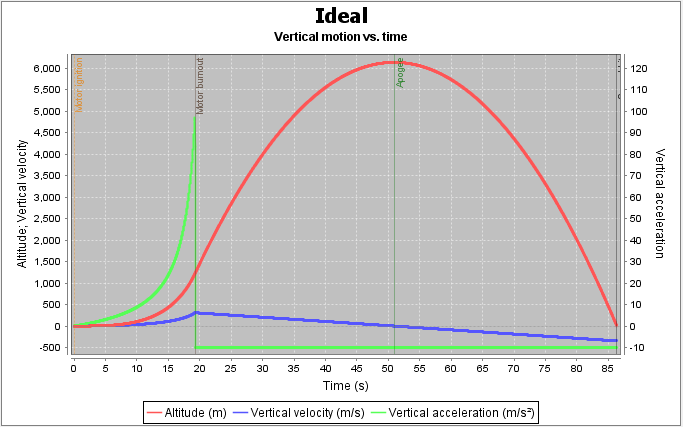
\includegraphics[width = 0.75\textwidth]{./figures/idealCurve.png}}
    \caption{OpenRocket Simulated Flight Results for Ideal Flight Case}
    \label{fig:idealCurve}
\end{figure}

\noindent Figure \ref{fig:idealCurve} shows the simulated ideal flight of the OpenRocket model where drag is ignored. 
The simulation results tells us that the maximum altitude achieved by the rocket is 6134 meters which closely matches the expected altitude of 6096 meters, resulting in a 0.60\% error.
The expected maximum velocity of the rocket was calculated to be 309.24 $\frac{m}{s}$.
The simulated flight returned a maximum velocity of 309.84 $\frac{m}{s}$, resulting in an error of 0.19\%.
The maximum normalized acceleration from the simulated flight was 9.89 which is very close to the expected value of 10, resulting in an error of 1.09\%.
This result tells us that the ideal flight case simulated in OpenRocket very closely matches our expected results.
This accuracy is due to us ignoring the drag component of the rocket's flight.\\

\begin{figure}[h!]
    \centering
    \fbox{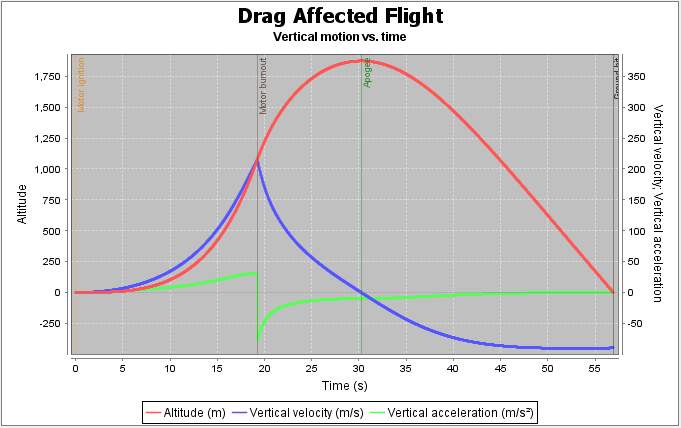
\includegraphics[width = 0.75\textwidth]{./figures/dragCurve.png}}
    \caption{OpenRocket Simulated Flight Results for Drag Affected Flight Case}
    \label{fig:dragCurve}
\end{figure}

\noindent Figure \ref{fig:dragCurve} shows the simulated flight of the OpenRocket model where drag is not ignored.
Comparing this figure to Fig. \ref{fig:idealCurve}, we can see that the drag drastically affected the rocket's maximum height, velocity, and acceleration.
The simulated maximum altitude of the drag affected flight was only 1874 meters, 69.26\% less than the expected value and 69.49\% less than the idealized case.
The maximum velocity of the drag affected flight was also lower at 215.31 $\frac{m}{s}$, 30.37\% less than the expected value and 30.51\% less than the idealized case.
The maximum normalized acceleration of the drag affected flight was not only lower at 7.96 but also in the negative direction due to drag stopping the rocket from climbing.
The maximum normalized acceleration of the flight was 20.39\% less than the expected value and 19.50\% less than the idealized case.
These results tell us that drag severely impacted the rocket's ability to fly, inhibiting the rocket's ability to reach even 50\% of the expected maximum altitude.
Because of this, this rocket does not satisfy baseline case conditions.
This result is expected because the equations used when configuring the rocket ignores the affect of drag.\\

\begin{figure}[h!]
    \centering
    \fbox{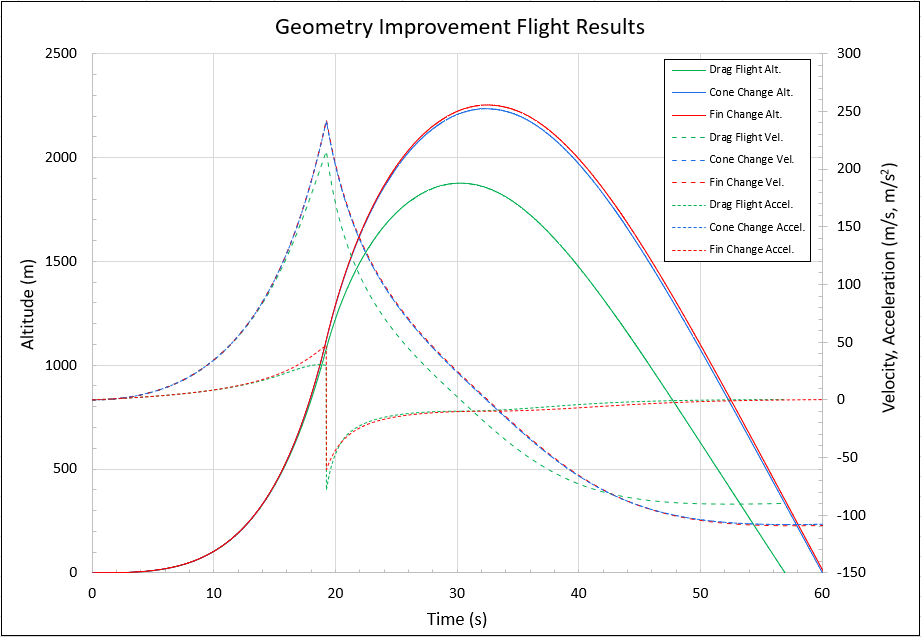
\includegraphics[width = 1\textwidth]{./figures/geoImprov.png}}
    \caption{Flight Results for Geometrically Improved Rocket}
    \label{fig:geoImprov}
\end{figure}

\noindent To achieve greater max. altitude without increasing the amount of propellant, improvements were made to the geometry of the rocket.
One of the improvements made to the rocket that also had the greatest impact was to switch the nose cone for one of a more aerodynamic shape.
Of the five choices available in OpenRocket, the Haack Series cone shape appears to improve the rocket the most.
From Fig. \ref{fig:geoImprov}, we can see that by switching the conical nose cone out for the Haack Series nose cone, the maximum altitude of the rocket increased from 1874 meters to 2235 meters, an increase of 19.26\%.
Another improvement made to the rocket was to give the fins of the rocket an airfoil cross-section and removing one of the fins, resulting in a three-fin design.
Although doing so changed the center of pressure and center of mass of the rocket, the change was very small at only 3.04\%.
With the changes in the fins, the maximum altitude of the OpenRocket model increased to 2253 meters, an improvement of 0.81\% from the previous and a total improvement of 20.22\% over the base design.
Like the maximum altitude, the max. velocity of the rocket increased from 215.31 $\frac{m}{s}$ to 242.73 $\frac{m}{s}$ (+12.74\%).
The max. acceleration of the rocket actually decreased due to the more aerodynamic design, decreasing from 7.96 to 6.16 (-22.76\%).\\

\begin{figure}[h!]
    \centering
    \fbox{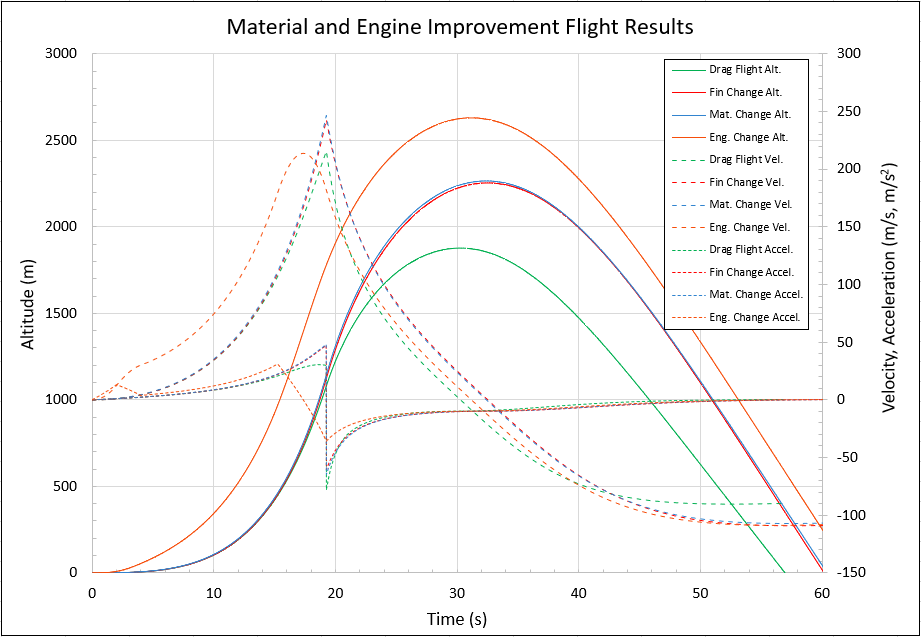
\includegraphics[width = 1\textwidth]{./figures/improv2.png}}
    \caption{Flight Results for Material and Engine Improved Rocket}
    \label{fig:improv2}
\end{figure}

\noindent To further improve our rocket, the rocket's material was also changed.
The purpose of changing the rocket's material is that lighter rockets require less force to accelerate.
Since our rocket was designed so that the shell doubles as the combustion chamber, the shell material must still be strong enough to hold all the internal pressure.
However, since only the area around the propellant have to be strong, the rest of the rocket can be made from a different material.
Instead of carbon-epoxy, the material for the rocket shell was changed to be balsa, a very light wood.
Compared to carbon-epoxy weighing at about 1.82 $\frac{g}{cm^3}$, balsa only weighs 0.17 $\frac{g}{cm^3}$, roughly 10 times less. 
We can see from Fig. \ref{fig:improv2} that changing the material of the rocket increased the maximum altitude of the rocket from 2253 meters to 2264 meters, an increase of 0.49\%.
This increase in maximum altitude is very small because the propellant was what contributed to most of the rocket's weight, not its shell.
The max. velocity and max. acceleration of the rocket increased slightly from 242.73 $\frac{m}{s}$ to 246.64 $\frac{m}{s}$ (+1.61\%) and 6.16 to 6.57 (+6.48\%) respectively.


\begin{figure}[h!]
    \centering
    \fbox{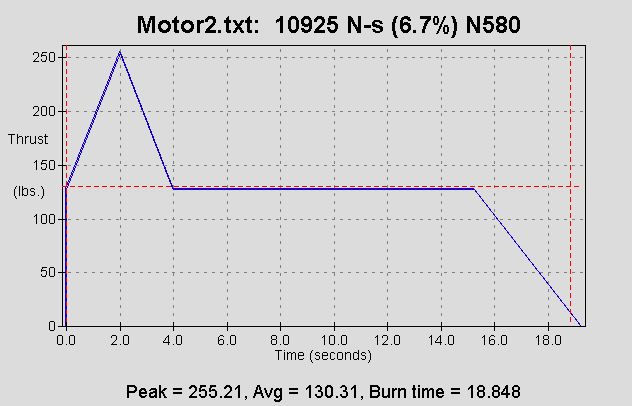
\includegraphics[width = .5\textwidth]{./figures/burnprof.png}}
    \caption{Burn Profile of New Engine}
    \label{fig:burnprof}
\end{figure}


\noindent The final improvement made to the rocket was to alter its burn-profile to make it more efficient.
A new burn profile was created where instead of a linear burn throughout the entire burn time, the propellant was burnt faster towards the launch and slower as the burn carries on.
Figure \ref{fig:burnprof} shows the burn profile of this new engine.
Although the new engine has the same impulse, propellant mass, and burn time as the old one, the new engine should be more efficient as less propellant is wasted trying to accelerate the rocket after it has gained speed, reducing fuel waste due to drag.
We can see from Fig. \ref{fig:improv2} that with the new burn profile, the rocket's max. altitude increased from 2264 meters to 2639 meters, an increase of 16.12\%.
The max. velocity and max. acceleration decreased from 246.64 $\frac{m}{s}$ to 213.64 $\frac{m}{s}$ (-13.38\%) and 6.57 to 6.65 (-44.45\%).
Although the max. velocity decreased, the rocket increased in velocity much sooner, allowing it to travel at fast speed for longer, resulting in greater altitude. 




\newpage
\section*{Appendix}
\addcontentsline{toc}{section}{Appendix}

\begin{equation}
    (C_{N\alpha})_n=2
\end{equation}

\begin{equation}
    \bar{X}_n = \frac{2L}{3}
\end{equation}

\begin{equation}
    (C_{N\alpha})_f = \frac{16}{1+\sqrt{1+(2.5D)^2}}
\end{equation}

\begin{equation}
    \bar{X}_f = L+D+\frac{D}{2}
\end{equation}

\begin{equation}
    k_{fb} = 1 + \frac{D}{3D}
\end{equation}

\begin{equation}
    X_{cp} = \frac{(C_{N\alpha})_n\bar{X}_n + k_{fb}(C_{N\alpha})_f\bar{X}_f}{(C_{N\alpha})_n+k_{fb(C_{N\alpha})_f}}
\end{equation}

\end{document}
